

%---%
\chapter{Elméleti Bevezető}
%---%

\section{Elméleti alapok}

\subsection{Posztulátumok: \cite{kvantkonyv1}} 
\underline{1.állapotteres leírás:} Egy zárt fizikai rendszer éppen aktuális állapota leírható egy \textbf{V} Hilbert tér-beli egységhosszú, komplex együtthatós állapotvektorral. Hilbert tér például egy komplex lineáris vektortér, amire értelmezve van a belső szorzat(skalárszorzat). 
Vegyünk példának egy két dimenziós Hilbert teret, ami egy egyszerű zárt fizikai rendszer jelképez. A rendszer állapotát le lehet írni egy /textbf{v} két dimenziós vektorral, ahol:\\
\begin{center}
$ v= \begin{bmatrix} a\\b \end{bmatrix} = a\textbf{0}+ b\textbf{1} $ ,ahol 
$\textbf{0}=\begin{bmatrix} 1\\0 \end{bmatrix} , \textbf{1}=\begin{bmatrix} 0\\1 \end{bmatrix} ,   a,b \in C$
\end{center}
Itt \textbf{0} és \textbf{1} az orthonormális(ortgonális és egyséhosszú) bázisvektorok. Mivel az állapotvektor egységhosszú,ezért ki kell még kötni, hogy 
$\abs{a}^2+\abs{b}^2 =1$ . Az együtthatókra szokás még valószínűségi amplitúdóként is hivatkozni(a Schrödinger hullámfüggvényben amplitúdóként jelennek meg).

\underline{2.Rendszerek időbeli fejlődése:}Zárt fizikai rendszer időbeli fejlődése leírható csak változás kezdő- és végpontjától függő unitér transzformációval. Az előbbi jelölésrendszer segítségével leírva: 
\begin{center}
$v'(t_2) = U(t_1,t_2)v(t_2), v' \in V$
\end{center}
$ U $ unitér operátor lineáris algebrai reprezentációja egy \textbf{U} kvadratikus mátrix, melynek $U_{ij}$ elemei a bemeneti \textbf{j} orthonormális bázisvektor \textbf{i} vektorral való kapcsolatát jelképező valószínűségi amplitúdókat jelölik.\\

\underline{3.Mérés:} Méréseket leírhatunk$M_m$  mérési operátorokkal, ahol $m$ a lehetséges mérési eredményeket jelöli. $m$ mérésének a valószínűsége, ha a rendszer \textbf{v} állapotban van:
\begin{center}
$P(m|\textbf{v})= {\textbf{v}}^\dagger M_m^\dagger M_m \textbf{v} $
\end{center}
A rendszer állapota mérés után:
\begin{center}
$ {\textbf{v}}' = \frac{M_m \textbf{v}}{\sqrt{{\textbf{v}}^\dagger M_m^\dagger M_m \textbf{v}}}  $
\end{center}
Mivel a kimenetek összesített valószínűsége 1-el egyenlő.(a lehetséges kimenetek lefedik a teljes eseményteret):
\begin{center}
$ \sum_m P(m|\textbf{v}) = \sum_m {\textbf{v}}^\dagger M_m^\dagger M_m \textbf{v} \equiv 1$
\end{center}
ami alapján:
\begin{center}
$\sum_m M_m^\dagger M_m \equiv I $
\end{center}
A mérések nem visszafordíthatóak és viszonylag durvának tekinthetőek abból a szempontból, hogy befolyásolják a mért rendszer állapotát a fentebb már leírt módon. Ugyanakkor velük teremthetjük meg a kapcsolatot a klasszikus és a kvantum világ között, mivel ők azok az eszközök,  amikkel megfigyelhetjük mégiscsak mi történik a kvantum világban.
\\
\underline{4.Összetett rendszerek:}
Egy $ W $ összetett fizikai rendszer állapota leírható az őt összetevő rendszerek tenzorszorzataként:
$ W=V \otimes Y $ .Továbbá ha $\textbf{v} \in V  $  és  $ \textbf{y} \in Y $ akkor a belőlük alkotott állapot: $ \textbf{w}=\textbf{v}\otimes \textbf{y} $ .
A kvantummechanikában a legkisebb információt hordozó elem a bit, amit kvantumbitnek, vagy röviden qubitnek  szokás hívni. Egy qubit szokványos leírása:
\begin{center}
$ \ket{\psi}=a\ket{0}+b\ket{1}=a \begin{bmatrix}1\\0\end{bmatrix}+ b \begin{bmatrix}0\\1\end{bmatrix} = \begin{bmatrix} a\\b \end{bmatrix} $
\end{center}
A klasszikus számítástechnikához hasonlóan n qubit felhasználásával építhetünk n bites kvantumregisztereket. Vizsgáljunk például egy két qubitből alkotott kvantumregisztert. Ekkor a teljes két qubites rendszer állapota:
\begin{center}
$ \ket{\psi} \equiv \ket{\psi_1}\ket{\psi_2} \equiv \ket{\psi_1,\psi_2} \equiv \ket{\psi_1\psi_2} $
\end{center}
Ami például hogyha:
\begin{center}
$ \ket{\psi_1} = \frac{\ket{0}+\ket{1}}{\sqrt{2}}, \ket{\psi_2}=\frac{\ket{0}+\ket{1}}{\sqrt{2}}, $
\end{center}
akkor:
\begin{center}
$ \ket{\psi}= \frac{\ket{0} \otimes \ket{0} +\ket{0}\otimes\ket{1}+\ket{1}\otimes\ket{0}+\ket{1}\otimes\ket{1}  }{2} = \frac{\ket{00}+\ket{01}+\ket{10}+\ket{11}}{2} $
\end{center}
látszik, hogy az előbbi rendszer a 00,01,10,11 állapotok(ők mellesleg ortogonálisak egymásra,itt az állapottér bázisának tekinthetőek) súlyozott(most itt mindegyik 1/2 -el de ez lehet bármilyen más komplex szám is, sőt akár 0 is.) összege, ezeket mind tartalmazza és jól látszik, hogy felbontható $\ket{\psi_1}$  és  $\ket{\psi_2}$  tenzorszorzatára. Az ilyen állapotokat hívjuk szorzat állapotoknak.\\
Most vizsgáljuk a következő állapotot:
\begin{center}
$ \ket{\psi} = a\ket{00}+b\ket{11} $
\end{center}
Ezt nem tudjuk felbontani két qubit tenzorszorzatára. Az ilyen állapotokat hívjuk összefonódott állapotnak. Vegyük észre ennek az állapotnak egy érdekes tulajdonságát. Ha megmérjük az egyik bitjét, akkor akkor valamilyen valószínűséggel 0-át vagy 1-et kapunk. Viszont ha ezután megmérjük a másik bitet is, ha az első mérésünk eredménye 0 volt, akkor itt már csak 0 mérhetünk és ehhez hasonlóan 1-es eredmény esetén pedig csak 1-et. Továbbá kísérletileg bizonyított, hogy ez a jelenség akkor is fenn marad, ha a rendszer két qubitjét helyileg egymástól eltávolítjuk.
Néhány nevezetes összefonódott állapot, amelyeket Bell-állapotoknak szokás nevezni:
\begin{center}
$ \ket{\Phi^-}= \frac{1}{\sqrt{2}}(\ket{0_A0_B}-\ket{1_A1_A}) $ \\
$ \ket{\Phi^+}= \frac{1}{\sqrt{2}}(\ket{0_A0_B}+\ket{1_A1_A}) $ \\
$ \ket{\Psi^-}= \frac{1}{\sqrt{2}}(\ket{0_A1_B}-\ket{1_A0_A}) $ \\
$ \ket{\Psi^+}= \frac{1}{\sqrt{2}}(\ket{0_A1_B}+\ket{1_A0_A}) $ \\

\end{center}

Figyeljük meg, hogy ezek az állapotok egymásra merőlegesek, az állapotérnek bázisaiként szolgálhatnak. Ennek segítségével definiálhatjuk az ún. Bell mérést ami egy 2 qubites rendszer projektív mérése ezekben a bázisokban. Megjegyzendő még, hogy a mérés után a mérési posztulátumnak megfelelően a két qubit a négy Bell állapot egyikébe kerül.\\
Ezeken felül, bár a továbbiakhoz nem feltétlen szükséges, viszont a hivatkozások olvasásához igen, ismerjünk meg a rendszerek egy másik lehetséges leírási módját a teljesség igénye nélkül, a sűrűségmátrixos leírást\cite{kvantkonyv2}. Ebben az esetben a rendszert a lehetséges állapotainak valószínűségeinek összegével jellemezzük:
\begin{center}
$ p=\sum_i p_i \ket{\phi}\bra{\phi_i} $
\end{center}
ahol $ \ket{\phi_i} $ az i-edik rendszer állapot, melynek előfordulási valószínűsége $ p_i $ a sűrűségmátrixos leírás ilyen ún. tiszta állapotok valószínűségi elegyeként írja le a rendszert.Ezek alapján például a 
\begin{center}
$ \ket{\psi}=a\ket{0}+b\ket{1}= \begin{bmatrix} a\\b \end{bmatrix} $
\end{center}
rendszer sűrűségmátrixa a következőképpen számolható:
\begin{center}
$ p= \ket{\phi}\bra{\phi} = \begin{bmatrix} a \\ b \end{bmatrix} = \begin{bmatrix} a* b* \end{bmatrix}= \begin{bmatrix} aa* ab*\\a*b bb* \end{bmatrix} = \begin{bmatrix} \abs{a}^2 ab* \\ a*b \abs{b}^2 \end{bmatrix} $
\end{center}
Ezen felül definiáljük még a “trace” (magyarul nyom) operátort a következőképpen. Egy n-szer n-es A mátrixra:
\begin{center}
$ Tr(A) = a_{11}+a_{22}+... +a_nn= \sum_{i=1}^n a_{ii} $
\end{center}
Továbbá említésre méltó még, hogy Tr(A) egyenlő A sajátértékeinek összegével.

\section{Összefonódás megosztás}
(entanglement swapping)
\subsection{A jelenség bemutatása}
Az összefonódott állapotok érdekes tulajdonságait, természetesen igyekszünk kihasználni a kvantuminformatikában is, nem véletlen tehát, hogy magára az összefonódásra is mint egy fontos erőforrásként tekinthetünk. Elég csak olyan, protokollokra gondolni, mint a szupersűrűségű kódolás, vagy a kvantumteleportáció, melyek mind összefonódott állapotok “használnak el” a működésük során.Nem csoda tehát,hogy egy adott helyen(vagy helyek között) való összefonódás létrehozásának képessége különös jelentőséggel bír. Ezzel kapcsolatban létezik szerencsére egy számunkra igen hasznos és viszonylag sokszor hasznosított jelenség, az összefonódás megosztás(entanglement swapping), mellyel egy összefonódott párok közötti érdekes interakciót írunk le. A már 1993-ban felvetett koncepció szerint\cite{zukowski1993event} 2 összefonódott pár interakcióját vizsgáljuk egymással a következő módon.A példában tekintsünk kvantum információ hordozóira fotonokként hivatkozunk, de természetesen minden fotonhoz hasonló kvantum információ hordozására hasznos módszerre is az alábbiak szerinti a jelenség. Az összefonódott párjaink közül az egyik kezdetben legyen Alíznál, a másik pedig Bobnál. Legyen a rendszerünk kezdő állapota:
\begin{center}
$ \ket{\Psi_{kezd}^-}= \ket{\Psi^-}_{AB} \otimes \ket{\Psi^-}_{CD} $
\end{center}
ahol $ \Psi^- $ a már fentebb említett Bell állapot,AB fotonpár van Alíznál és CB fotonpár pedig Bobnál.A teljes állapot felírható:
\begin{center}
$ \ket{\Psi_{kezd}^-} = \frac{1}{2} \Big( \ket{\Psi^+}_{AD}\ket{\Psi^+}_{BC}-\ket{\Psi^-}_{AD}\ket{\Psi^-}_{BC} - \ket{\Phi^+}_{AD}\ket{\Phi^+}_{BC}+\ket{\Phi^-}_{AD}\ket{\Phi^-}_{BC} \Big) $
\end{center}
Alíz elküldi A fotont Bobnak, Bob pedig C fotont Alíznak, tehát Alíznál lesz B és C, míg Bobnál A és D. Ha Alíz Bell mérést hajt végre BC fotonpárján és $ \ket{\Psi^-}_{BC} $  állapotban találja, akkor ha Bob is megméri a saját párját $ \ket{\Psi^-}_{AD} $ állapotot fog találni. Ha Alíz a mérése során a maradék három állapot közül találja valamelyiket, akkor Bob ennek megfelelő állapotokat fog találni az ő fotonpárja mérésénél is. Látszik, hogy a Bobnál előfordulható állapotok mind tiszta összefonódott állapotok, emiatt ha Alíz Bell mérést végez, tudhatjuk, hogy a Bobnál lévő fotonpár össze van fonódva Alíz mérési eredményének pontos ismerete nélkül. Érdemes megfigyelni, hogy a Bobnál lévő fotonok semmilyen közös múlttal nem rendelkeznek, mégis szert tettek egy közös tulajdonságra, összefonódott állapotba kerültek.
A folyamatot lehet úgy is tekinteni, mintha a kvantumteleportációs protokoll\cite{bennett1993teleporting} segítségével egy már kezdetben is összefonódott állapot egyik kvantumbitjét teleportáltuk volna, csak ebben az esetben nem a kiválasztott kvantumbit pontos átvitele a fontos, hanem csak az összefonódás, mint a két kvantumbites rendszerre jellemző állapot, továbbítása az. Alíz mérési eredményének pontos ismerete és a feltételes visszaállító transzformációk, továbbá az ehhez szükséges 2 klasszikus bitnyi információ itt nem is része  a folyamatnak, mivel fentebb már megmutattuk, hogy az összefonódás léte(ami most minket érdekel) ezek nélkül is belátható.
\\
\begin{figure}[H]
\centering
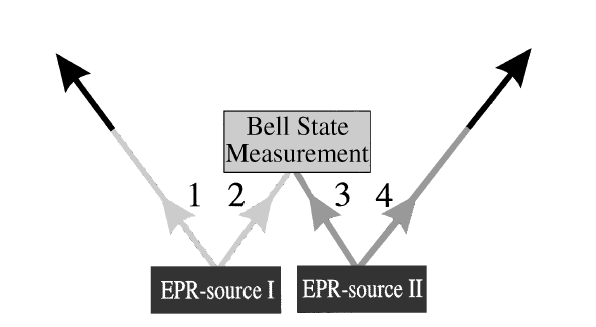
\includegraphics[width=120mm, keepaspectratio]{osszfonmeg1}
\caption[Összefonódás megosztás elvi rajza]{Összefonódás megosztás elvi rajza: Két összefonódott pár forrás (EPR source I és II) összefonódott fotonpárokat bocsájt ki(1-2 és 3-4). Mindegyik párból 1-1 fotonnal (2 és 3) végrehajtunk egy közös Bell mérést, aminek hatására a maradék két foton(1 és 4) is összefonódott állapotba kerül.}
\end{figure}
Megjegyzendő még érdekességként, hogy Peres elméletének megfelelően\cite{peres2000delayed} az összefonódás megosztás akkor is végbemehet, ha a (jelen esetben Alíznál) Bell mérést csak azután hajtjuk végre, hogy Bobnál már megmértük a másik két(jelen példánál A és D) állapotokat. Ezt igazolja például egy 2012-es kísérlet is\cite{ma2012experimental}.
\\
\begin{figure}[H]
\centering
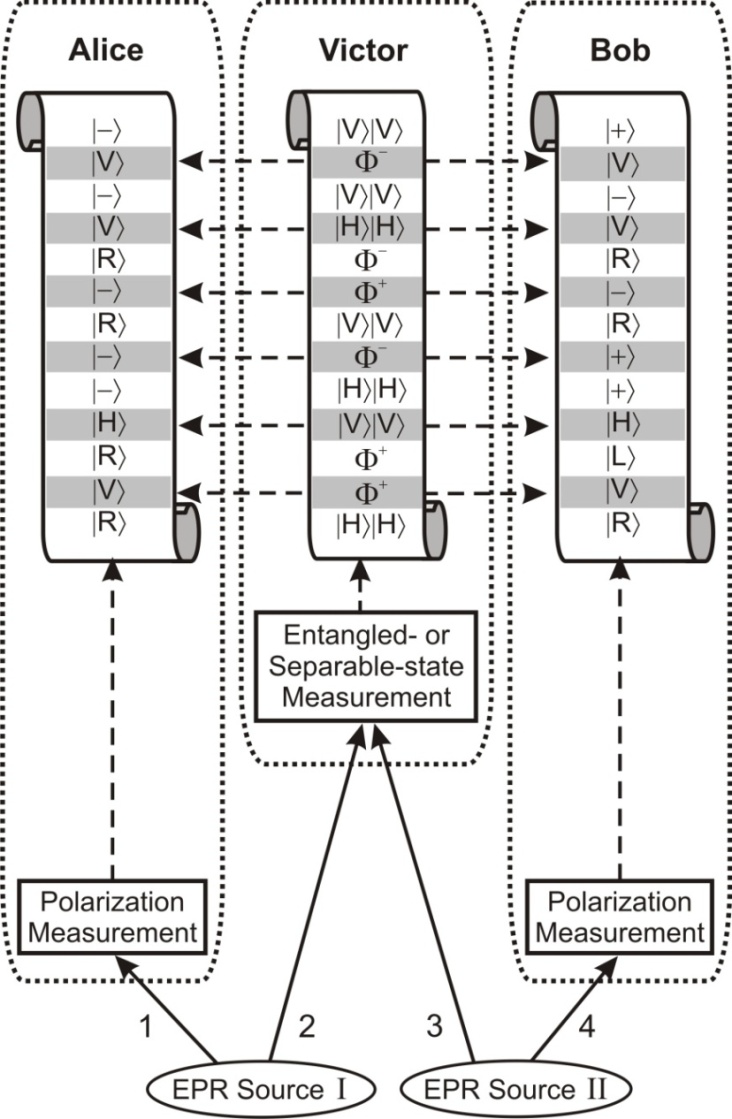
\includegraphics[width=120mm,keepaspectratio]{delayedchoice}
\caption[Késleltetett összefonódás megosztás kísérlet]{Elvi kísérleti összeállítás delayed choice(késleltetett döntéses) összefonódás megosztás vizsgálatára. Az előzőekhez hasonlóan itt is két összefonódott pár forrás szolgáltatja a fotonpárokat, viszont a korábbiakkal ellentétben itt először az 1-es és 4-es foton állapotait nézzük meg, utána véletlenszerűen döntünk, hogy Bell mérést, vagy valamilyen szétválasztható állapot szerinti mérést végzünk el. Ezek után Alice és Bob rendezni és vizsgálni tudja a már meglévő mérési adatait Victor döntése ismeretében. Azt kapjuk, hogy Alice és Bob fotonjai vagy összefonódott vagy szétválasztható állapotokként viselkednek, Victor mérési eredményeinek megfelelően.}
\end{figure}

\subsection{Összefonódás megosztások összefűzése}

Tekintve, hogy milyen fontos szerepe van az összefonódásnak a kvantumkommunikáció területén, az összefonódás megosztás is egy fontos eljárása, építőeleme számos kvantumkommunikációs protokollnak. Ezek közül talán az egyik legfontosabb ilyen felhasználási terület a kvantum ismétlők. A kvantumkommunikációs csatornák a valóságban nem tekinthetőek tökéletesnek, hasonlóan a klasszikus összeköttetésekhez, itt is számolni kell például csillapítással(hosszabb távon komoly probléma például a fotonok elnyelődése, detektálásuk nehézsége), a környezet hatásaival, mint például dekoherencia,zaj. Ebből adódóan nem élhetünk azzal a feltételezéssel, hogy hosszabb kapcsolatoknál az elküldött információnk a fogadó oldalra eredet formájában jut el. A kvantum csatorna átvitelére jellemző exponenciális csökkenés pedig gyakorlatilag ellehetetleníti a hosszabb távokon át történő információátvitelt. Erre lehetne az egyik megoldás, a klasszikus kommunikációhoz hasonlóan, ha megfelelően nem túl nagy távolságonként ismételnénk, eredeti állapotában mindig újra küldenénk tisztábban. A klasszikus kommunikációban ez könnyedén megoldható, azonban a kvantumos másolási tétel (No Cloning Theory) miatt nem lehet azt a megoldást teljes egészében lemásolni.Vegyük észre viszont, hogy a kvantum teleportációs protokoll segítségével tetszőleges állapotot tudunk elvinni egyik helyről a másikra, feltéve hogy a cél és a forrás rendelkezik egy összefonódott párral amin már előzőleg megosztottak.A problémát ily módon vissza tudjuk vezetni összefonódott párok szétosztására(mert klasszikus információt már tudunk nagy távolságokra is szállítani).Összefonódott párokat különben sem csak a teleportációs protokoll használ működése során, két hely közötti összefonódásra tekinthetünk egy általában is értékes erőforrásként. Itt lehet segítségünkre az összefonódás megosztás jelentősége.  
 
Természetesen az összefonódott párokat akarunk szétosztani ugyanúgy fennállnak az előzőleg említett problémák a csatornával, viszont tekintsük a következő esetet\cite{goebel2008multistage}: Ha az összefonódott párok közül az egyiket előzőleg összefonódás megosztásával hozzuk létre, könnyen elképzelhető, egy szabadon bővíthet séma, ahol a nagy átviteli távolságot, többszöri összefonódás megosztásával több kisebb szakaszra lehet bontani.
Vizsgáljuk meg azt az esetet amikor ezt a hosszabb távot két részre osztjuk fel. Ilyenkor kétszer kell összefonódást megosztani, három összefonódás forrásunk van, és két Bell mérést hajtunk végre a párjaink. Ha a párjaink kezdetben 1-2 3-4 és 5-6, akkor a Bell méréseket hajtunk végre 2-3-on és 4-5-ön. Ennek eredményeként 1 és 6 kerül összefonódott állapotba.
\\

\begin{figure}[h!]
\centering
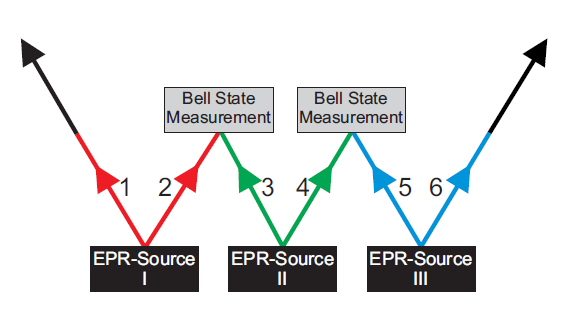
\includegraphics[width=120mm,keepaspectratio]{swapconcat}
\caption[Összefonódás megosztások összefűzése]{Többlépcsős összefonódás megosztás elvi felépítése:\\
A források által(EPR-Source I-II-III) kiadott kezdeti összefonódott párok: 1-2, 3-4, 5-6. 2 és 3-on majd 4 és 5-ön elvégezzük a Bell mérést. A két Bell mérés hatására végül 1 és 6 kerül összefonódott állapotba.}
\end{figure}

Felírva a rendszer állapotát:
\begin{center}
$ \ket{\Psi}_{123456}= \ket{\Psi^-}_{12} \otimes \ket{\Psi^-}_{34} \otimes \ket{\Psi^-}_{56} $
\end{center}
Ez átírható a következő alakra:
\begin{center}
$ \ket{\Psi}_{123456} = \frac{1}{2} \Big[ \ket{\Psi^+}_{14}\ket{\Psi^+}_{23}-\ket{\Psi^-}_{14}\ket{\Psi^-}_{23}-\ket{\Phi^+}_{14}\ket{\Phi^+}_{23} + \ket{\Phi^-}_{14}\ket{\Phi^-}_{23} \Big] \otimes \ket{\Psi^-}_{56} $
\end{center}
A korábbi két fotonpáros esethez hasonlóan itt is megfigyelhető, hogy az 1-es és 4-es fotonok a Bell mérés után összefonódott állapotban lesznek a mérés eredményétől függetlenül. Az eredmény csak arról szolgáltat információt, hogy melyik összefonódott állapotban vannak,, mivel az most is egyezik 2-3 közös mért állapotával.
Ha feltesszük, hogy 2-3-as fotonpárnál $ \ket{\Phi^-} $   állapotot mértünk, a fennmaradó 4 fotonos rendszer a továbbiakban a következő formában írható fel:
\begin{center}
$ \ket{\Psi}_{1456} = \frac{1}{2}\Big[ \ket{\Psi^+}_{16}\ket{\Phi^-}_{45}+\ket{\Psi^-}_{16}\ket{\Phi^+}_{45} - \ket{\Phi^+}_{16}\ket{\Psi^-}_{45} - \ket{\Phi^-}_{16}\ket{\Psi^+}_{45} \Big] $
\end{center}
Hasonlóan az előzőekhez, elvégezzük a Bell mérést 4-5-ön, aminek hatására 1 és 6 összefonódott állapotba kerül. A mérési eredménynek megfelelően például, ha a Bell mérésnél $\ket{\Phi^-} $ állapotot mérünk, akkor 1-6-nak az állapota: $ \ket{\Psi^+} . $ \\
A folyamat a fentiekből kiindulva általánosítható több tetszőleges számú összefonódott párral, tetszőleges számú Bell-méréssel, amivel az áthidalni kívánt távolság is tetszőleges számú szakaszra bontható fel.\\
A itt ábrázolt módszer is még idealizált csatornákkal dolgozik, magában nem oldja az előzőleg említett problémákat, mégis egy fontos építőeleme a későbbi ismétlő létrehozására irányuló modelleknek.
%%%
\subsection{A kvantum ismétlő}
%%%
A kvantum ismétlő megvalósítására törekvő modellek túlnyomó része három fő építőelemből áll, és jellemzően e három építőelem más és más megvalósításában tér el egymástól.Egy jellemző általános megvalósítás az alábbi:
A nagy távolságon jelentkező romlás elkerülése végett, ezt a távolságot felosztjuk több kisebbre, amik között a fentebb részletezett módon összefonódás megosztással teremtünk kapcsolatot. A felosztott kis távolságok között állomásokat alakítunk ki(ismétlőket), itt végezzük el az összefonódás megosztáshoz szükséges Bell méréseket. Továbbá minden szakaszhoz(minden összefonódás megosztási lépcsőhöz) létre kell hoznunk plusz összefonódott párokat amiket a folyamat során elhasználunk. Ehhez szükségünk van egy összefonódott pár forrásra, ami manapság már igen sokféle lehet[].Ez az egyik fő hasonlóság és egyben különbség is a legtöbb megvalósításban. A csatorna nem ideális átvitelével még mindig nem foglalkoztunk, pedig látható, hogy az továbbra is exponenciálisan fog romlani a csomópontok és a hossz növelésével. Ennek kiküszöbölésére használhatunk valamilyen összefonódás tisztító eljárást. Ezek jellemzően több nem teljesen tiszta összefonódott állapotból állítanak elő kevesebb, tisztább, jobban összefonódott állapotok.Tipikusan van egy tisztasági határérték a felhasznált “koszos” összefonódott állapotokra ami fölött alkalmazhatóak, emiatt akár ezek paraméterei támaszthatnak határokat a csatornaszakaszok hossza felé. Segítségükkel az átviteli sebesség kárára ugyan, de az átviteli folyamatok közé megfelelően beiktatva, kompenzálhatóak a csatornából származó veszteségek. \\
\underline{Példa egy tisztító protokollra}\\
Egy lehetséges ilyen tisztító protokoll például a Bennett által javasolt[8] aminek folyamán helyben végzett transzformációk segítségével több nem teljesen “tiszta” összefonódott párból kevesebb jobban összefonódott állapot hozható létre. (Megemlítendő, hogy eredetileg elektronspinekre írták le, de természetesen megvalósítható más hordozók esetén is.) Legyen M egy “kevert”(nem tiszta) állapot amiből tisztább, jobban összefonódott állapotokat szeretnénk létrehozni. (Ilyen lehet például egy zajos csatornán megosztott $ \ket{\Psi^-} $  pár.) Ilyenkor M tisztaságát az eredeti teljesen összefonódott állapothoz képest 




